\section{Overall description}
	\subsection{Product perspective}
        In terms of perspective, our product is the most important part of a larger system. The larger system includes three parts, and which are importing data, managing data and analysing data, so main functionality of the product are used to import and manage data. The product is dependent on other parts of whole system because this product will relate to other services on AWS such as S3 as data storage and DynamoDB as database. On the other hand, we need to complete basic reporting and analysing function. Hence there should be data transmission between database and data analytics.
        
        \begin{figure}[h]
        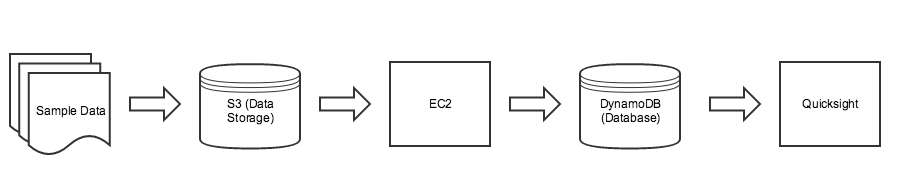
\includegraphics[width=18cm, height=4cm]{work_flow.png}
        \centering
        \caption{work flow of entire system}
        \end{figure}
        
	\subsection{Hardware Interface} 
       The database is built on public cloud so AWS platform will provide all aspects of the hardware supports. For example, high capacity solid state disks will used to store data items as a storage of product. And low-latency network connection can ensure maximum speed of accessing database.

	\subsection{Software interface}
        The AWS platform contains a variety of software provisioning for our product. On the one hand, developers can use proper programming language to implement functions of product base on via SDKs provided by AWS. On the other hand, the management console can help developer monitor all kinds of condition of database such as calculating throughput and cost. 
       
 	\subsection{Production function}
       The product will store different types of data such as log file, clickstream data in database. Besides, the product will provide enough space to hold vast amount of data, and it is able to build index and process data in batch. Furthermore, the database will implement some basic operations including inserting, deleting, updating and searching for data. Eventually, analysis technical will communicate to database, and then data will be accessed quickly by analysis technical while all of valuable data will be used to represent behaviors of students and staffs.

	\subsection{User characteristics}
        There is only one type of user that interact with our product: data analyzer. Staff who analyze the data can insert different types of data into database. Then, they could search the information base on the specific condition. After searching, data analyzer could do some management for the data such as sorting data. Finally, data analyzer could also extract the data from database and load it into a data analysis tool to do the analysis. 

	\subsection{Constraints}
        In implementation, there are minimal constraints placed on design. There are, however, certain aspects of development that we must keep in mind, including resource limits, implementation language, and development environment. The main aspect being that development on the AWS platform will cost our client money. AWS charges for computing time, temporary data storage, and database usage. Though it is unlikely that we will run into any upper budget limit, we need to have in mind the charges in order to eliminate resource waste. Amazon also offers a budget tool for our client to track our budget usage. It can also provide a forecast for future budget, so we can know in advance if we are approaching any limit. In terms of implementation language, AWS is flexible in the choice of coding language; we are free to choose any programming language that they support. Finally, our development will be done from our personal machines; as a cloud computing service, Amazon’s resources can be freely accessed by us wherever on any operating system.

	\subsection{Assumptions and dependencies}
        Because the nature of the project is to produce a prototype of a cloud-based big data archive, there is an assumption that our final product will be a competitive solution for OSU’s data analytics, compared to a locally-hosted solution. From this base-assumption, there are several dependencies to keep in mind, including scalability, future maintenance, and security.\\ 
        
        \noindent Our development will be done mostly with small test-sets of data, with student information anonymized before given to us. Therefore, a large concern is scalability - our solution must be able to work with potentially enormous data sets in a reasonable time. Database retrieval time is critical; the solution is almost useless if it takes an inappropriately long time to extract data from our implemented database. Additionally, database manipulation time, such as “joins” is an important factor when considering adopting the final product. Other metrics will be determined as we begin design implementation.
    